\begin{center}
    \setcounter{section}{4}
    \section*{CAPÍTULO IV}
    \addcontentsline{toc}{section}{MARCO METODOLÓGICO}
    \vspace*{0.5in}
    \textbf{MARCO METODOLÓGICO}
\end{center}
\setcounter{subsection}{0}

\subsection{Identificación del sistema}
    Se planteo el monitoreo de un edificio el cual es alimentado con tres fases desde la empresa que suministra energía. 
    A través de un sistema SCADA mostrar variables
    asociadas al consumo generando un histórico que permita obtener valores, en consecuencia obtener
    a partir de este el costo asociado. Las variables del sistema a medir son las siguientes:
    \subsubsection{Variables del sistema}
    \begin{enumerate}
        \item \textbf{Edificio residencial:}

        \begin{itemize}
            \item \textbf{Tensión fase neutro:} Es la tensión suministrada desde el proveedor a la estructura con tres lineas fase
            neutro.
            \item \textbf{Tensión fase neutro promedio:} Es la tensión obtenida al sacar el promedio de las tensiones fase neutro.
            \item \textbf{Tensión fase fase:} Es el valor que se obtiene al medir la tensión entre dos fases.
            \item \textbf{Tensión fase fase prmedio:} Es el valor que se obtiene al obtener el promedio de la tensión fase fase medida anteriormente.
            \item \textbf{Corriente de línea:} Es la corriente suministrada por la central a través de una de las fases, monitorear
            este dato nos puede arrojar que sucede al momento de ocurrir una falla en el circuito.
            \item \textbf{Demanda instantánea activa:} Es la potencia consumida en una de las lineas que provienen desde el 
            distribuidor de energía por norma esta son habitualmente 3 fases generando la potencia activa de la linea uno, dos 
            y tres.
            \item \textbf{Demanda instantánea  activa total:} Se requiere medir y generar un histórico de la potencia instantánea consumida 
            por el conjunto completo, este valor está asociado a la potencia consumida total el cual se define como la suma de 
            la potencia consumida en las 3 fases que alimenta a la infraestructura. 
            \item \textbf{Factor de potencia:} Esta relación nos indica que la corriente consumida se consume e potencia activa 
            manteniendo la corriente en valores calculados.
            \item \textbf{Máxima demanda:} Es la máxima potencia consumida durante un periodo de tiempo.
            \item \textbf{Energía total:} Es la energía consumida referida por defecto a la anterior fecha de pago, con la posibilidad 
            de obtener en función de otro periodo de tiempo definido por el usuario. 
            \item \textbf{Costo total:} Es el costo de la energía consumida desde la anterior fecha de corte.
        \end{itemize}
        Estas variables tienen valores variables instantáneos, es posible generar un historial a través al almacenarlos en una 
        base de datos para mostrarlos en forma grafica.

        \item \textbf{Valores de un apartamento:}
        
        \begin{itemize}
            \item \textbf{Tensión de linea promedio:} Se obtiene al calcular el promedio de las tensiones fase neutro que recibe el inmueble.
            \item \textbf{Demanda activa total:} Es el consumo intantaneo de potencia activa consumida por el inmueble.
            \item \textbf{Energía consumida:} Es la energía consumida por el inmueble durante un periodo de tiempo.
            \item \textbf{Costo acumulado:} Es el costo asociado a la energía consumida.
            \item \textbf{Proxima fecha de pago:} Es la fecha asociada a la proxima fecha de corte de la energía consumida.
            \item \textbf{Estado de conexón:} Valor booleano asociado a la conexión o desconexión del servicio de energía.
        \end{itemize}
    \end{enumerate}
\subsection{Diseño de la estructura de la interfaz}

    En el diseño previo se empleo Adobe XD un software enfocado en el desarrolo UX/UI sin ser requerido el desarrollo del producto para
    poder visualizar la interfaz y la interacción con el usuario. Teniendo en cuenta el tamaño en px disponible en el software de MANGO AUTOMATION
    empleando herramientas de desarrollo en el buscador Chrome obteniendo de allí los colores bases y los tamaños estandares para el dieño.\\

    Se diseñan las siguientes insterfaces:\\
    \begin{itemize}

        \item \textbf{Overview:} Se plantea una interfaz (Figura \ref{figInterfazOverview}) en la cual se tiene la ubicación geografica de los edificios
        en monitoreo donde se presenta la información del nombre del edificio, demanda instantánea, Energía total acumulada y el costo total asociado al 
        consumo de energía consumida. Pensando en el monitoreo de distintos edificios permitiendo hacer uso de la plataforma en la administración de
        distintos condominios por parte de una empresa.

        \begin{figure}[H]
            \centering
                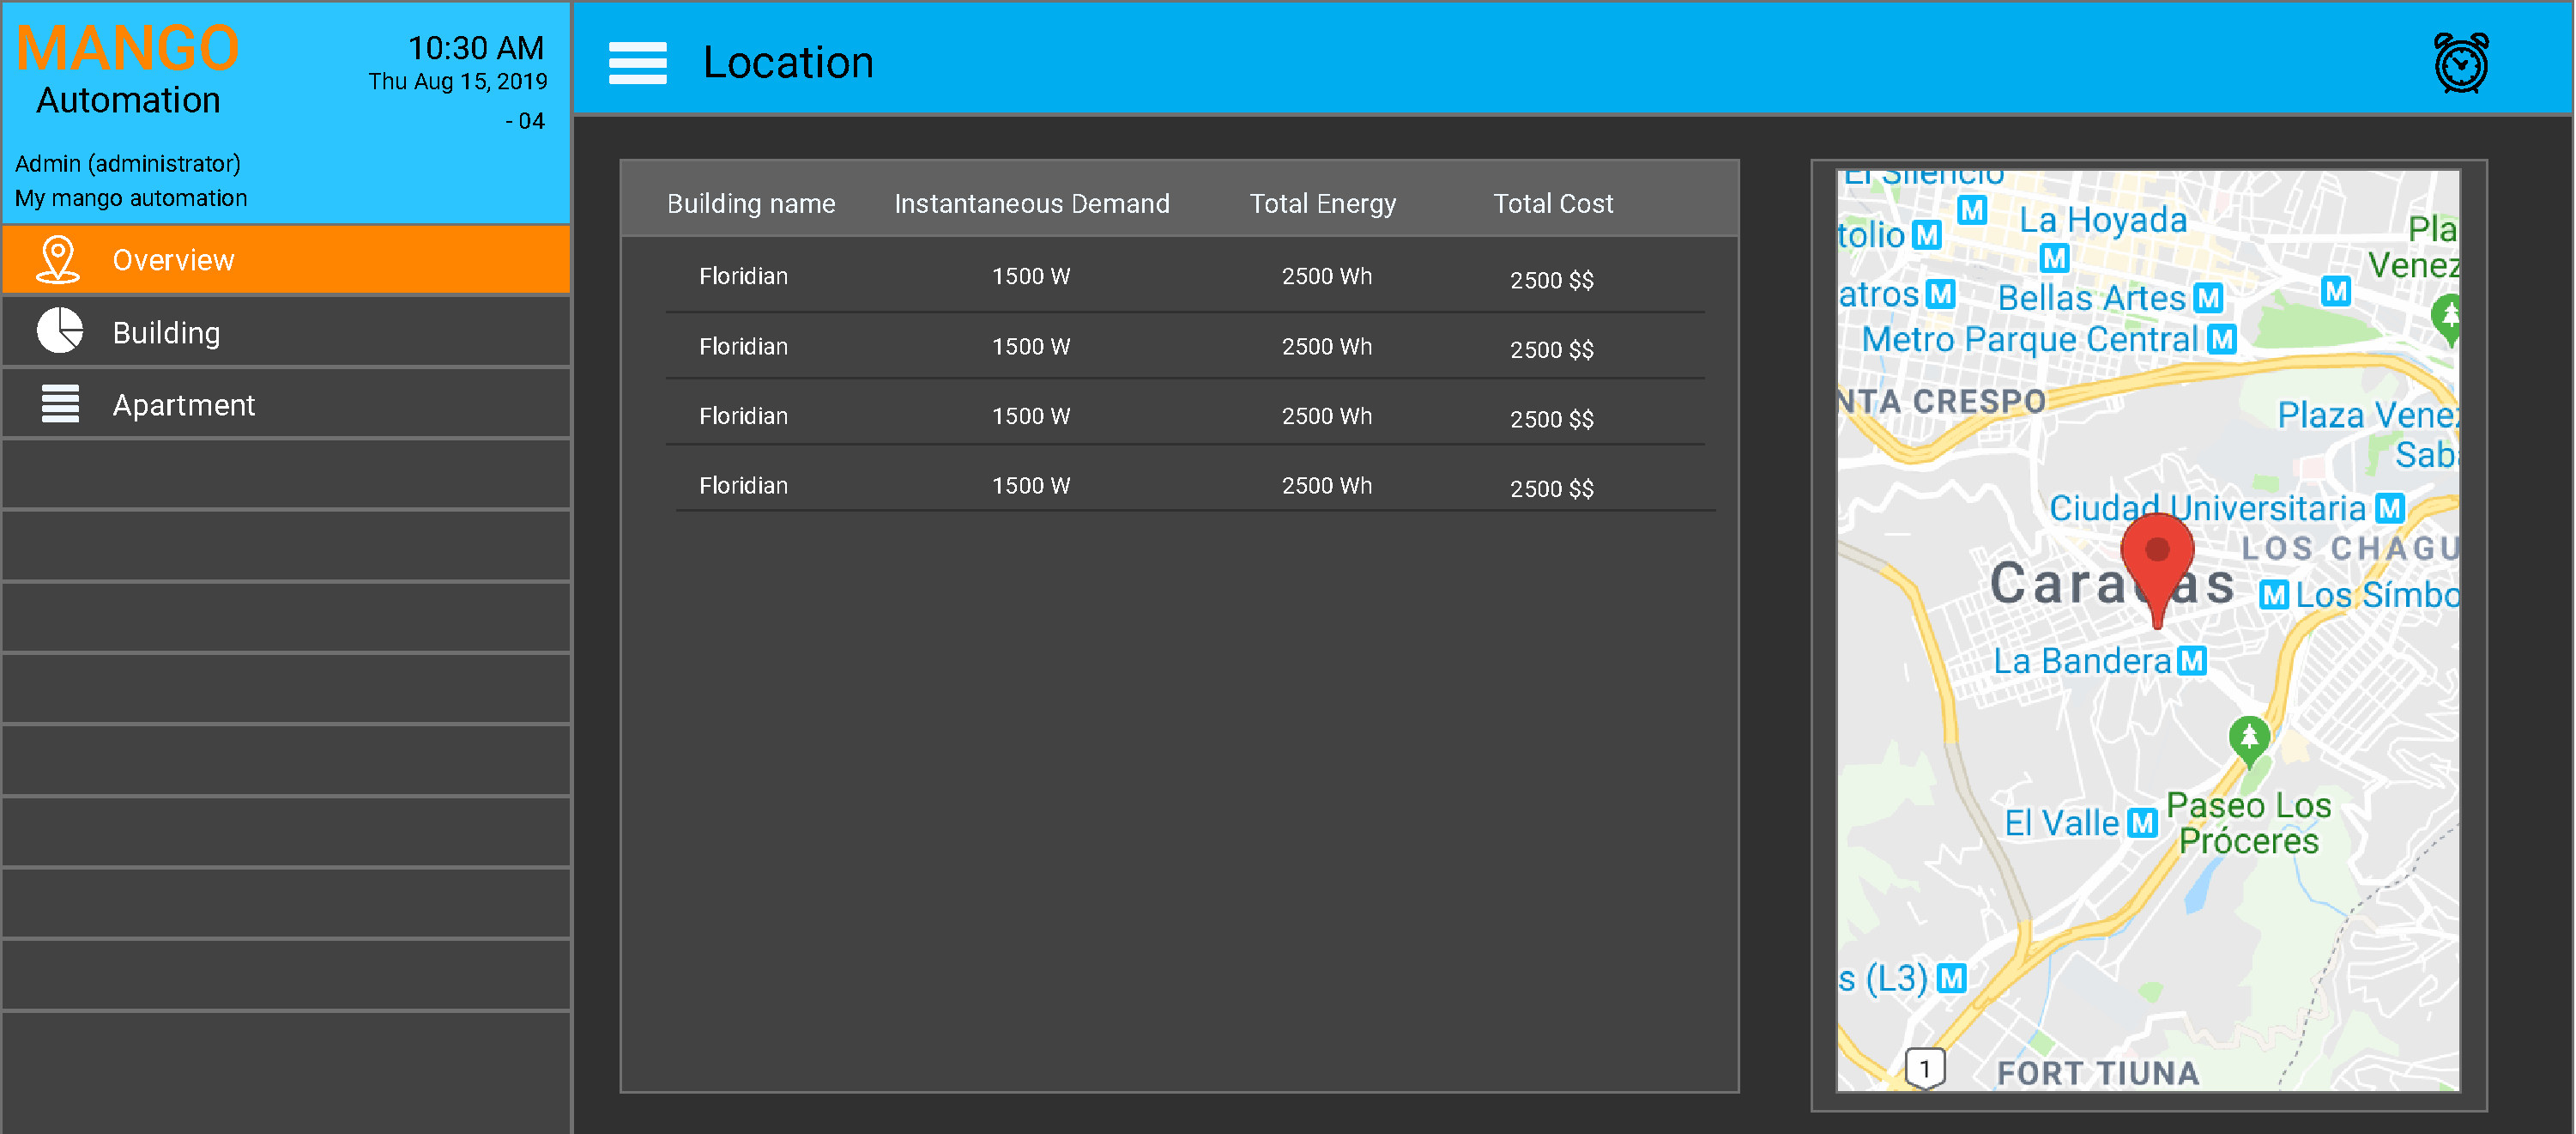
\includegraphics[scale=0.2]
                {overview.pdf}
            \caption{Interfaz overview}
            \label{figInterfazOverview}
        \end{figure} 
        
        \item \textbf{Building:} Se plantea una interfaz (Figura \ref{figInterfazBuilding}) donde se hace enfoque a cuatro variables Demanda Instantánea, Demanda Máxima, Energía Total y 
        Costo total enfocándose en parametros claves de costo y consumo.
        
        \begin{figure}[H]
            \centering
                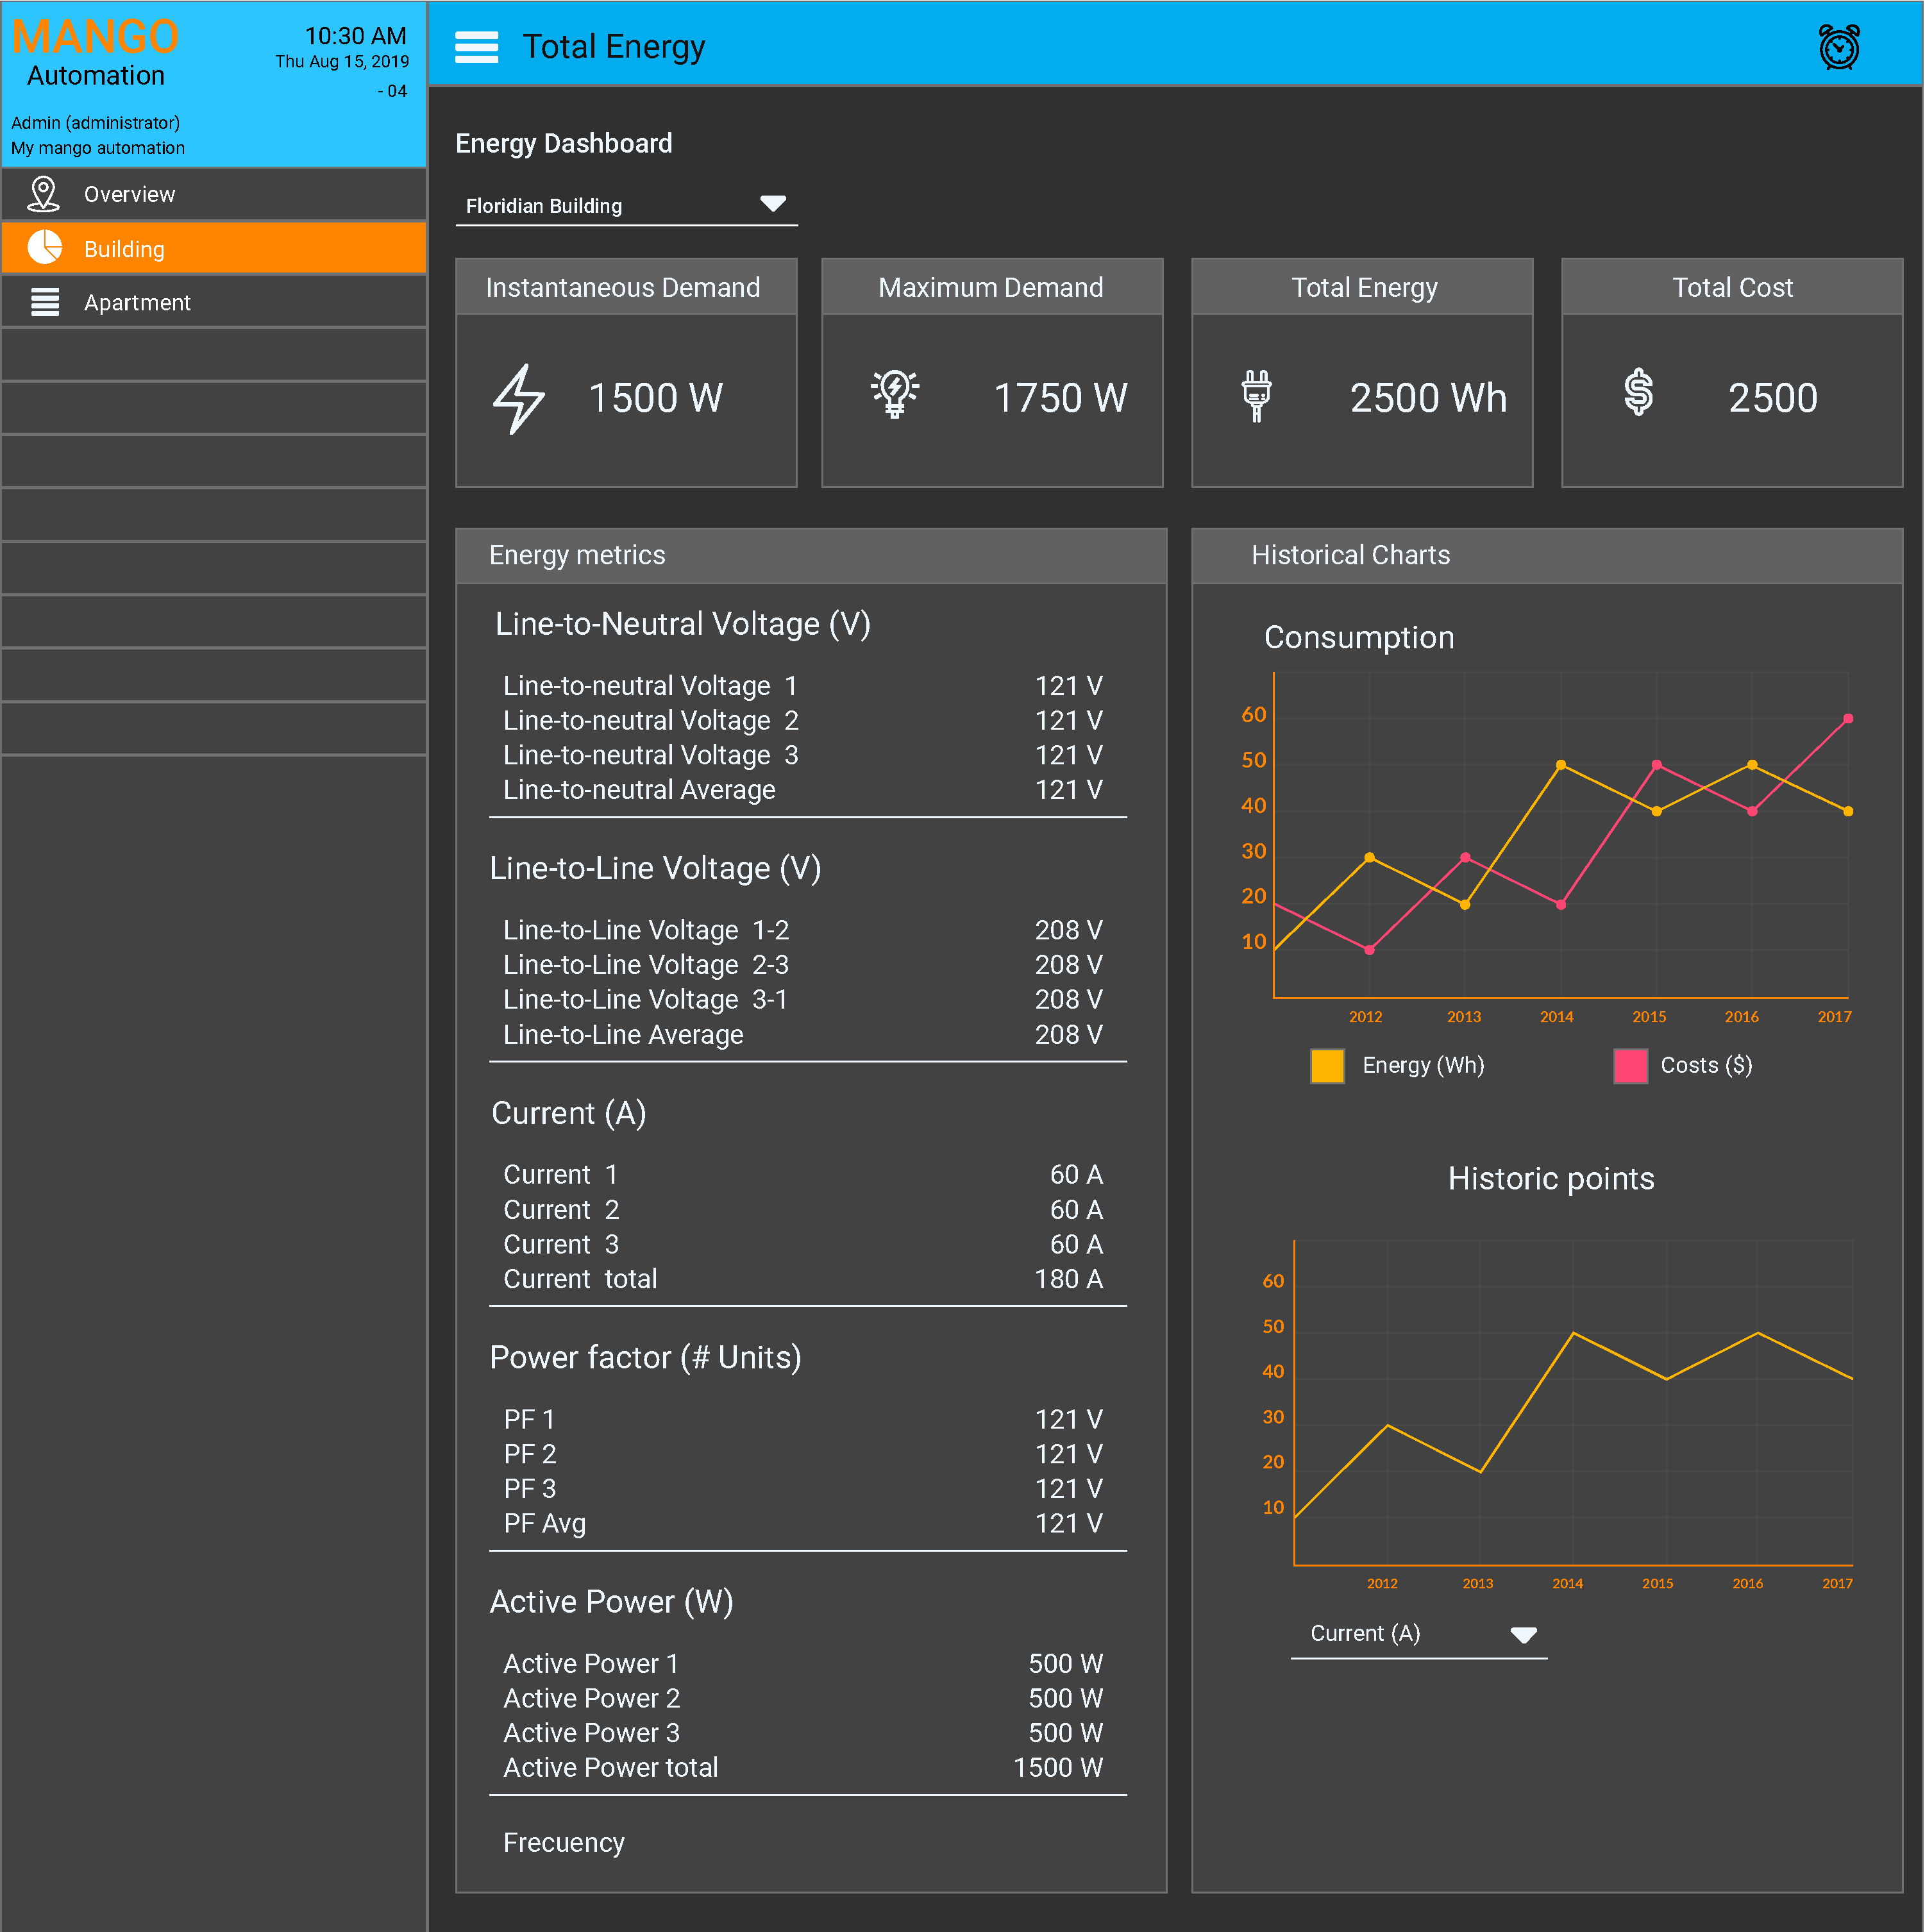
\includegraphics[scale=0.2]
                {building.pdf}
            \caption{Interfaz building}
            \label{figInterfazBuilding}
        \end{figure}

        Se diseñan dos bloques de información un primer asociado a las metricas instantánea con valores que permiten el monitoreo con valores de tensión, corriente,
        potencia, factor de potencia y frecuencia de la red y un segundo de bloque en donde se plantean graficas de la data obtenida a través del tiempo.
        Se estructura de tal manera que a primera vista con fines de administración financiera se obtiene la data importante para tal actividad, en caso de requerir
        monitoreo tecnico se presenta la información requerida para una rapida toma de decisiones o un analísis del sistema a través del tiempo.
 
        \item \textbf{Apartment:} Se plantea una interfaz (Figura \ref{figInterfazApartment}) el cual esta pensado para el usuario final y datos requeridos
        para estudios tecnicos por parte de un tecnico. Se presentan datos a la energía consumida, el costo asociado, la próxima fecha de pago, 
        y pagos retrasados, valores económicos importantes para el usuario que paga la cuenta de energía electrica además de valores que permitan 
        realizar estudios en caso de ser requeridos.

        \begin{figure}[H]
            \centering
                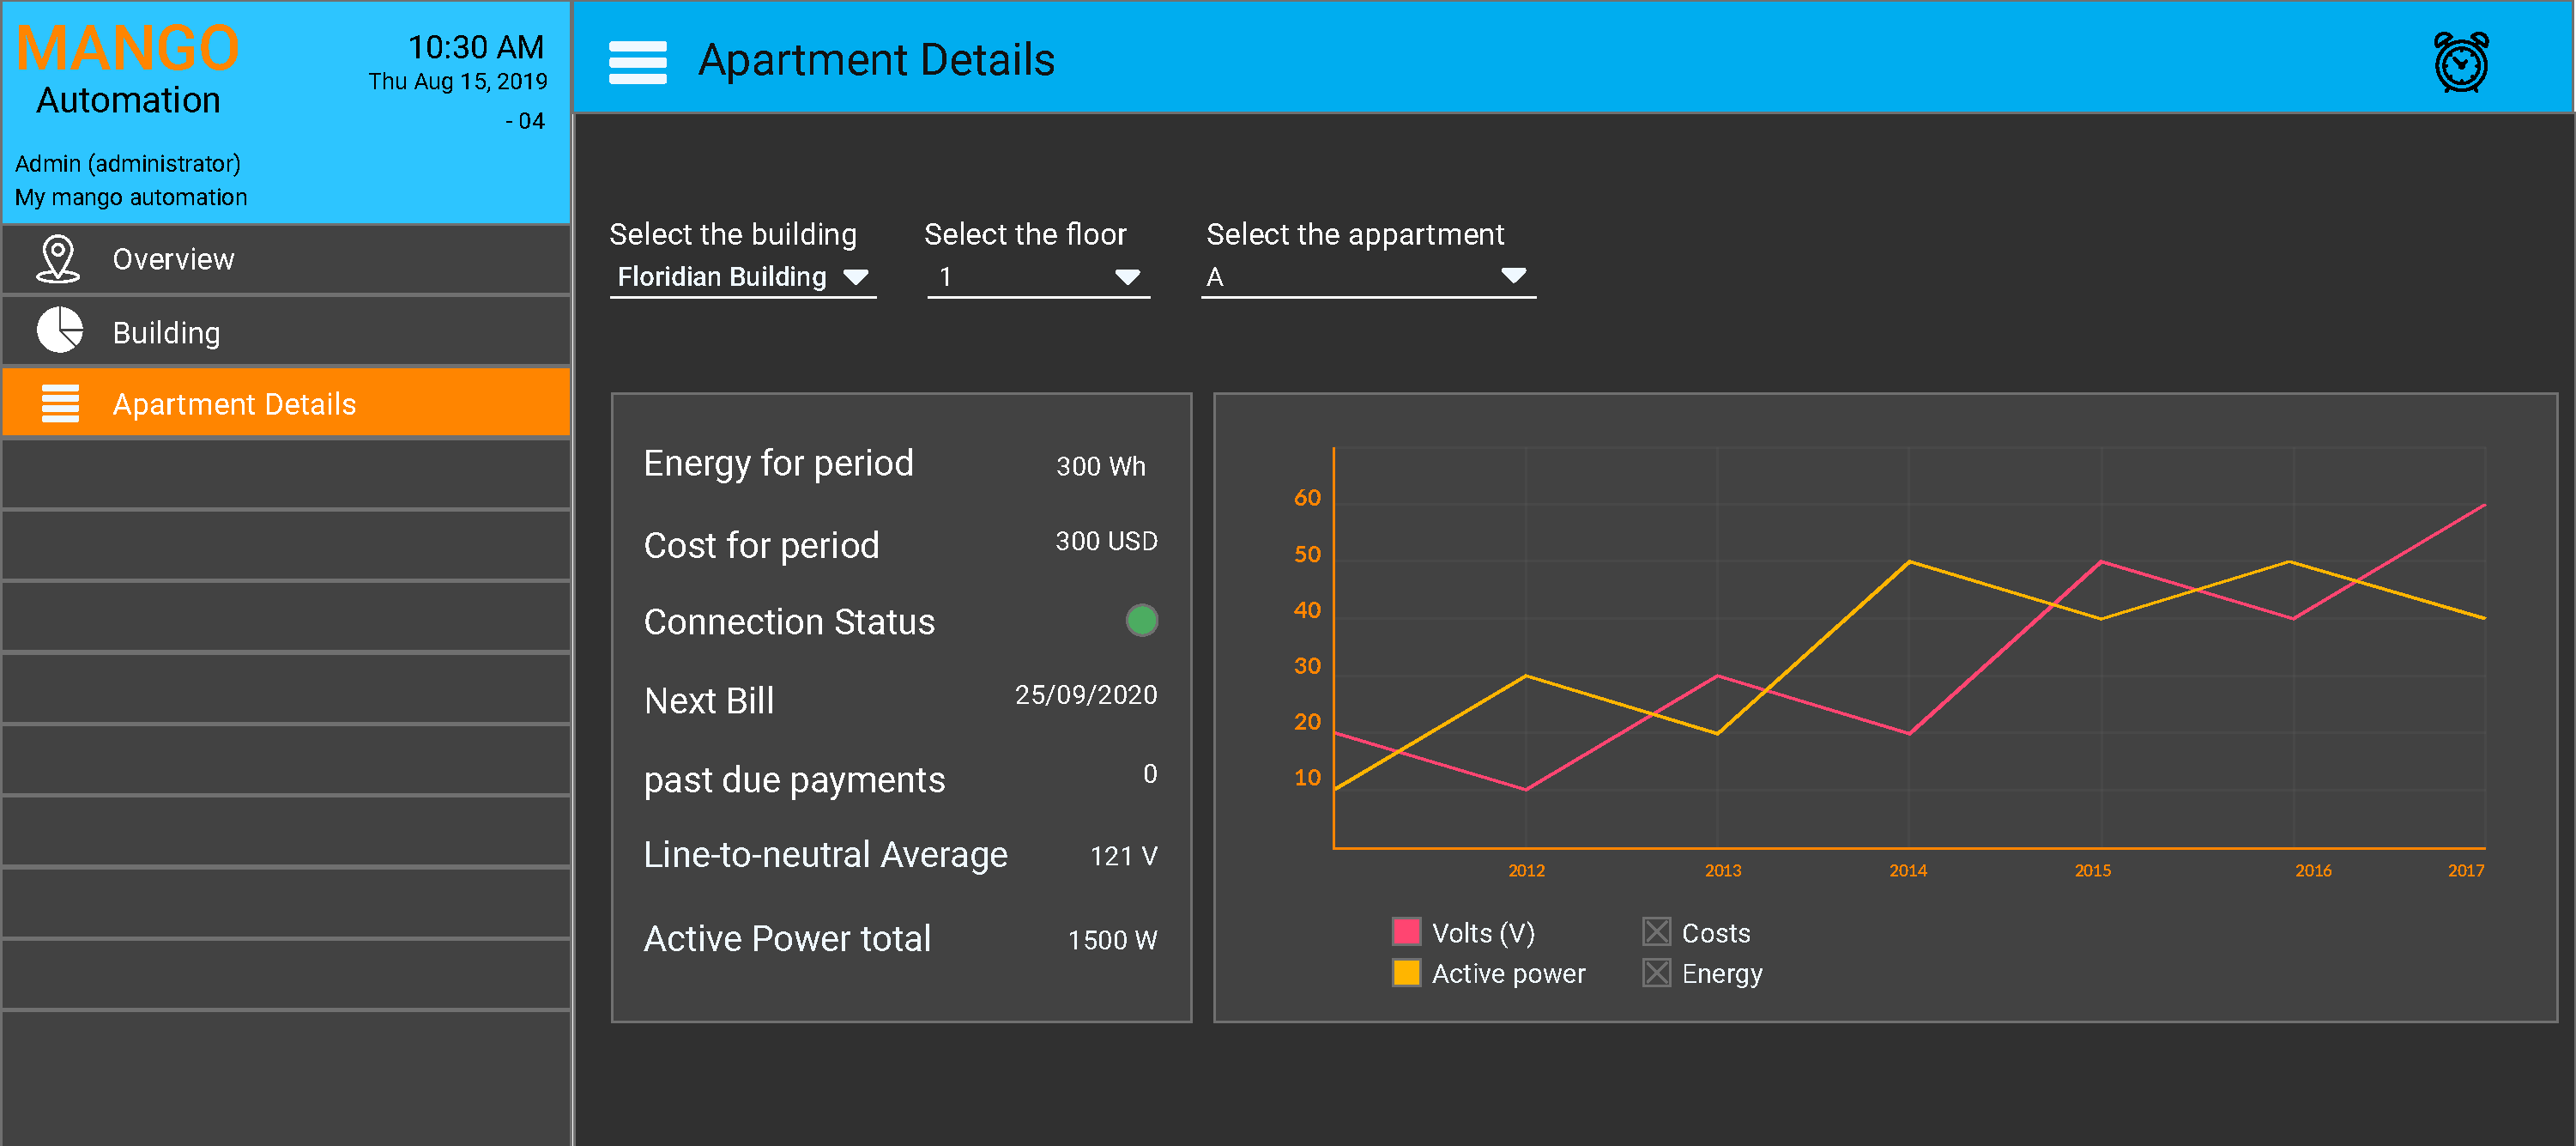
\includegraphics[scale=0.2]
                {apartment.pdf}
            \caption{Interfaz apartament}
            \label{figInterfazApartment}
        \end{figure}
    \end{itemize}
\subsection{Definición de Variables en plataforma de Mango AUTOMATION}
    La plataforma permite definir variables con el protocolo de comunicación a establecer, en nuetro caso se emplean Virtual Data Point 
    y meta Data source, la primera para generar de forma aleatoria da
\subsection{Desarrollo de la interfaz}
    
\newpage